\subsection{Modello di Dominio}
Scala party è un videogioco single-player, ispirato a "Mario Party",
famoso videogioco della Nintendo. In questa versione, i personaggi 
sono rappresentati da due pedine: una per il giocatore e l'altra per
l'avversario (computer). Tirando i dadi, il giocatore e il computer 
si muovono su un tabellone composto da caselle con l'obiettivo di
raccogliere il maggior numero di pioli, ovvero elementi collezionabili
che appariranno casualmente sul tabellone. Alla fine di ogni round,
il giocatore dovrà affrontare un minigioco single-player che permetterà
di ottenere dei vantaggi nel turno successivo.


Allo scopo di istruire il lettore sul funzionamento del sistema,
in questa sezione approfondiremo i seguenti aspetti:
\begin{enumerate}
    \item Le entità principali del dominio e le loro relazioni
    \item Le regole del gioco
\end{enumerate}
\subsubsection{Entità del Dominio}
\begin{figure}[h!]
\centering
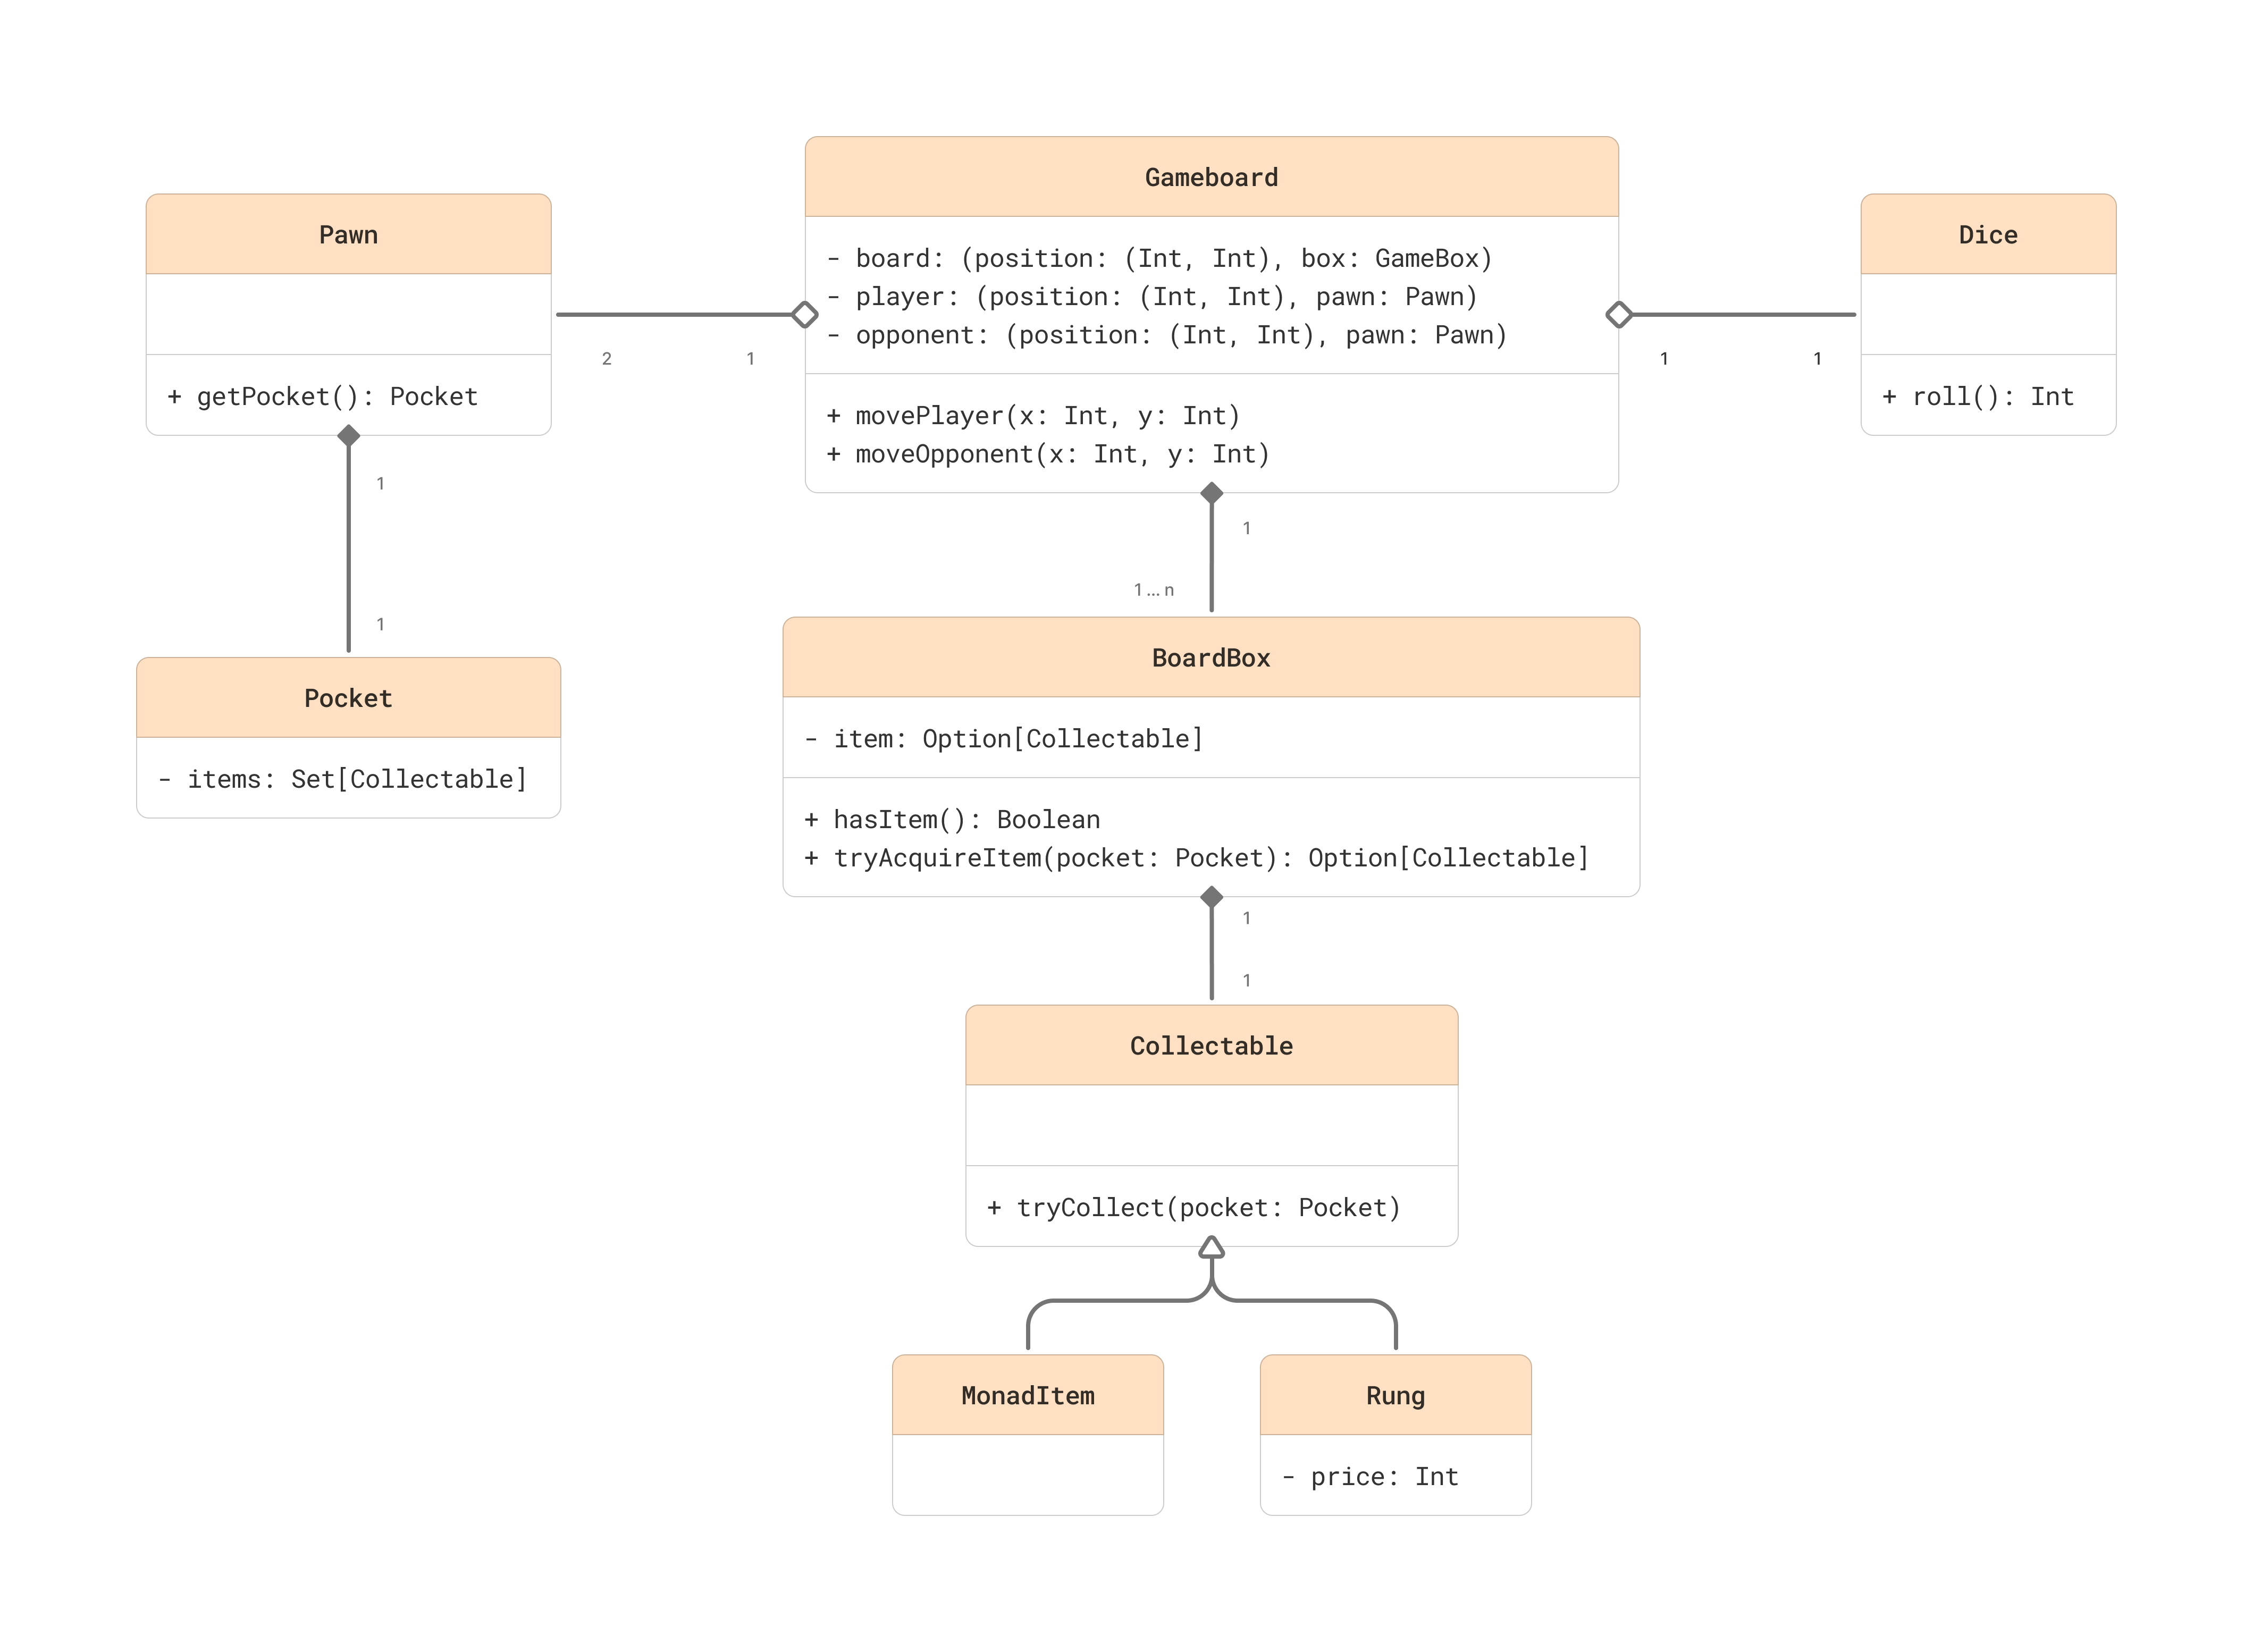
\includegraphics[width=1\textwidth]{figures/domain-class-diagram.png}
\caption{Diagramma delle Classi del Dominio}
\label{fig:domain-class-diagram}
\end{figure}
Approfondiamo le entità modellate nel diagramma delle classi 
a figura \ref{fig:domain-class-diagram}.
\begin{itemize}
    \item \textbf{Gameboard}\par
    \item \textbf{Board Box}\par
    \item \textbf{Dice}\par
    \item \textbf{Pawn}\par
    \item \textbf{Pocket}\par
    \item \textbf{Collectable}\par
    \item \textbf{MonadItem}\par
    \item \textbf{Rung}\par
\end{itemize}

\subsubsection{Regole del Gioco}